Prvi korak u analizi argumentacije je prepoznavanje, strukturiranje i 
izrada argumenata iz argumentativne rasprave \citep{scheuer2010computer,
prudencio2005visualizing}. Razvojem softvera za argumentaciju, 
olakšala se i analiza argumentacije. Prema \cite{Chris2017-REETAW}, Araucaria
je najpopularniji softver za analizu argumentaciju s 10000 korisnika iz
preko 80 zemalja između 2001. i 2010. godine. Upravo je Arauciaria
prvi alat koji je nastojao biti agnostičan na teoriju argumentacije
pretpostavljajući Toulminov model argumenta, zadržavajući kompatibilnost
s Wigmoreovim \citep{wigmore2016wigmore} i 
Freemanovim \citep{freeman1991dialectics} modelima. 
Zbog toga se Araucia smatra začetnikom Argument Weba. Araucaria je 
danas \footnote{7.1.2018. dostupna na URL-u \url{http://ova.arg-tech.org/}} 
dostupna online pod imenom OVA \engl{Online Visualization of Argument}. 

\section{Kolaborativna analiza}

\begin{figure}
\centering
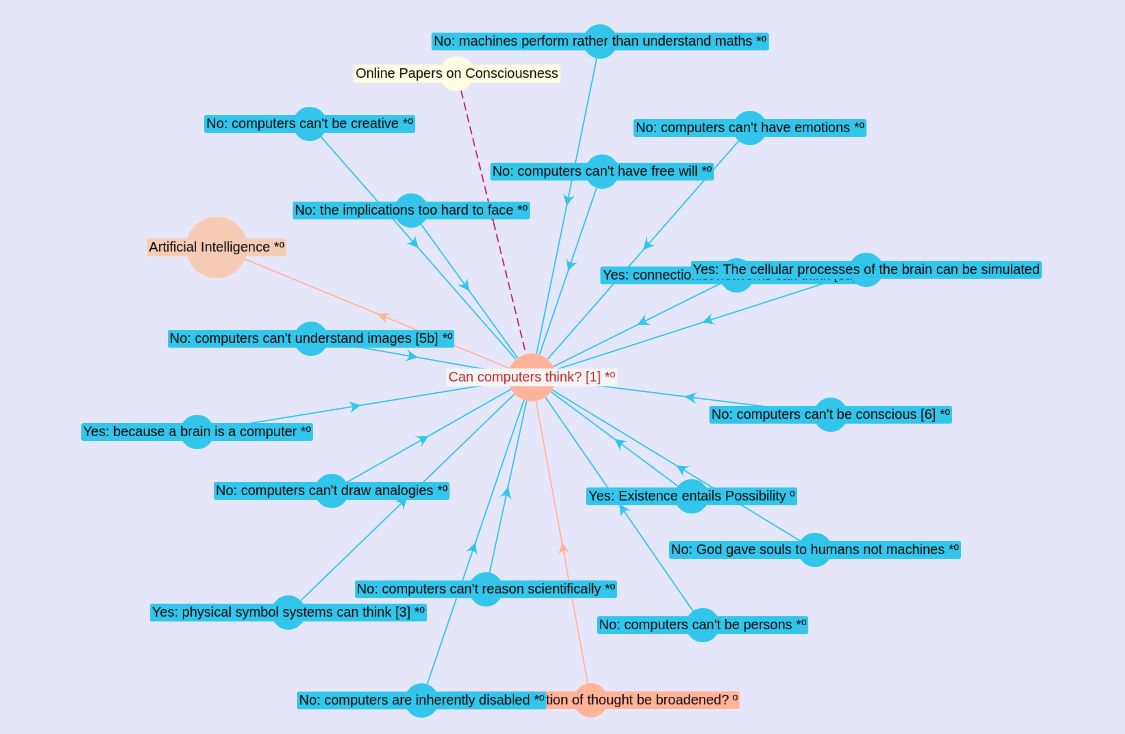
\includegraphics[scale=0.4]{debategraph.png}
\caption{Analiza mogu li računala razmišljati na DebateGraphu}
\label{fig:computers}
\end{figure}

Postavljanje sustava za analizu argumenata online olakšalo je suradnju 
na analizi argumentacije koja je neophodna u slučaju kompleksnije
argumentacije. Uz OVA alat, pojavili su se i drugi online alati za
analizu argumentacije. DebateGraph \footnote{7.1.2018. dostupno na 
\url{https://www.debategraph.com}} omogućava korisnicima hijerarhijsku 
analizu teme kroz grafove. Primjer na slici \ref{fig:computers} prikazuje
analizu \emph{Mogu li računala razmišljati} u sustavu DebateGraph. Svaki
čvor u grafu moguće je dodatno otvoriti i zasebno istražiti. 

\begin{figure}
\centering
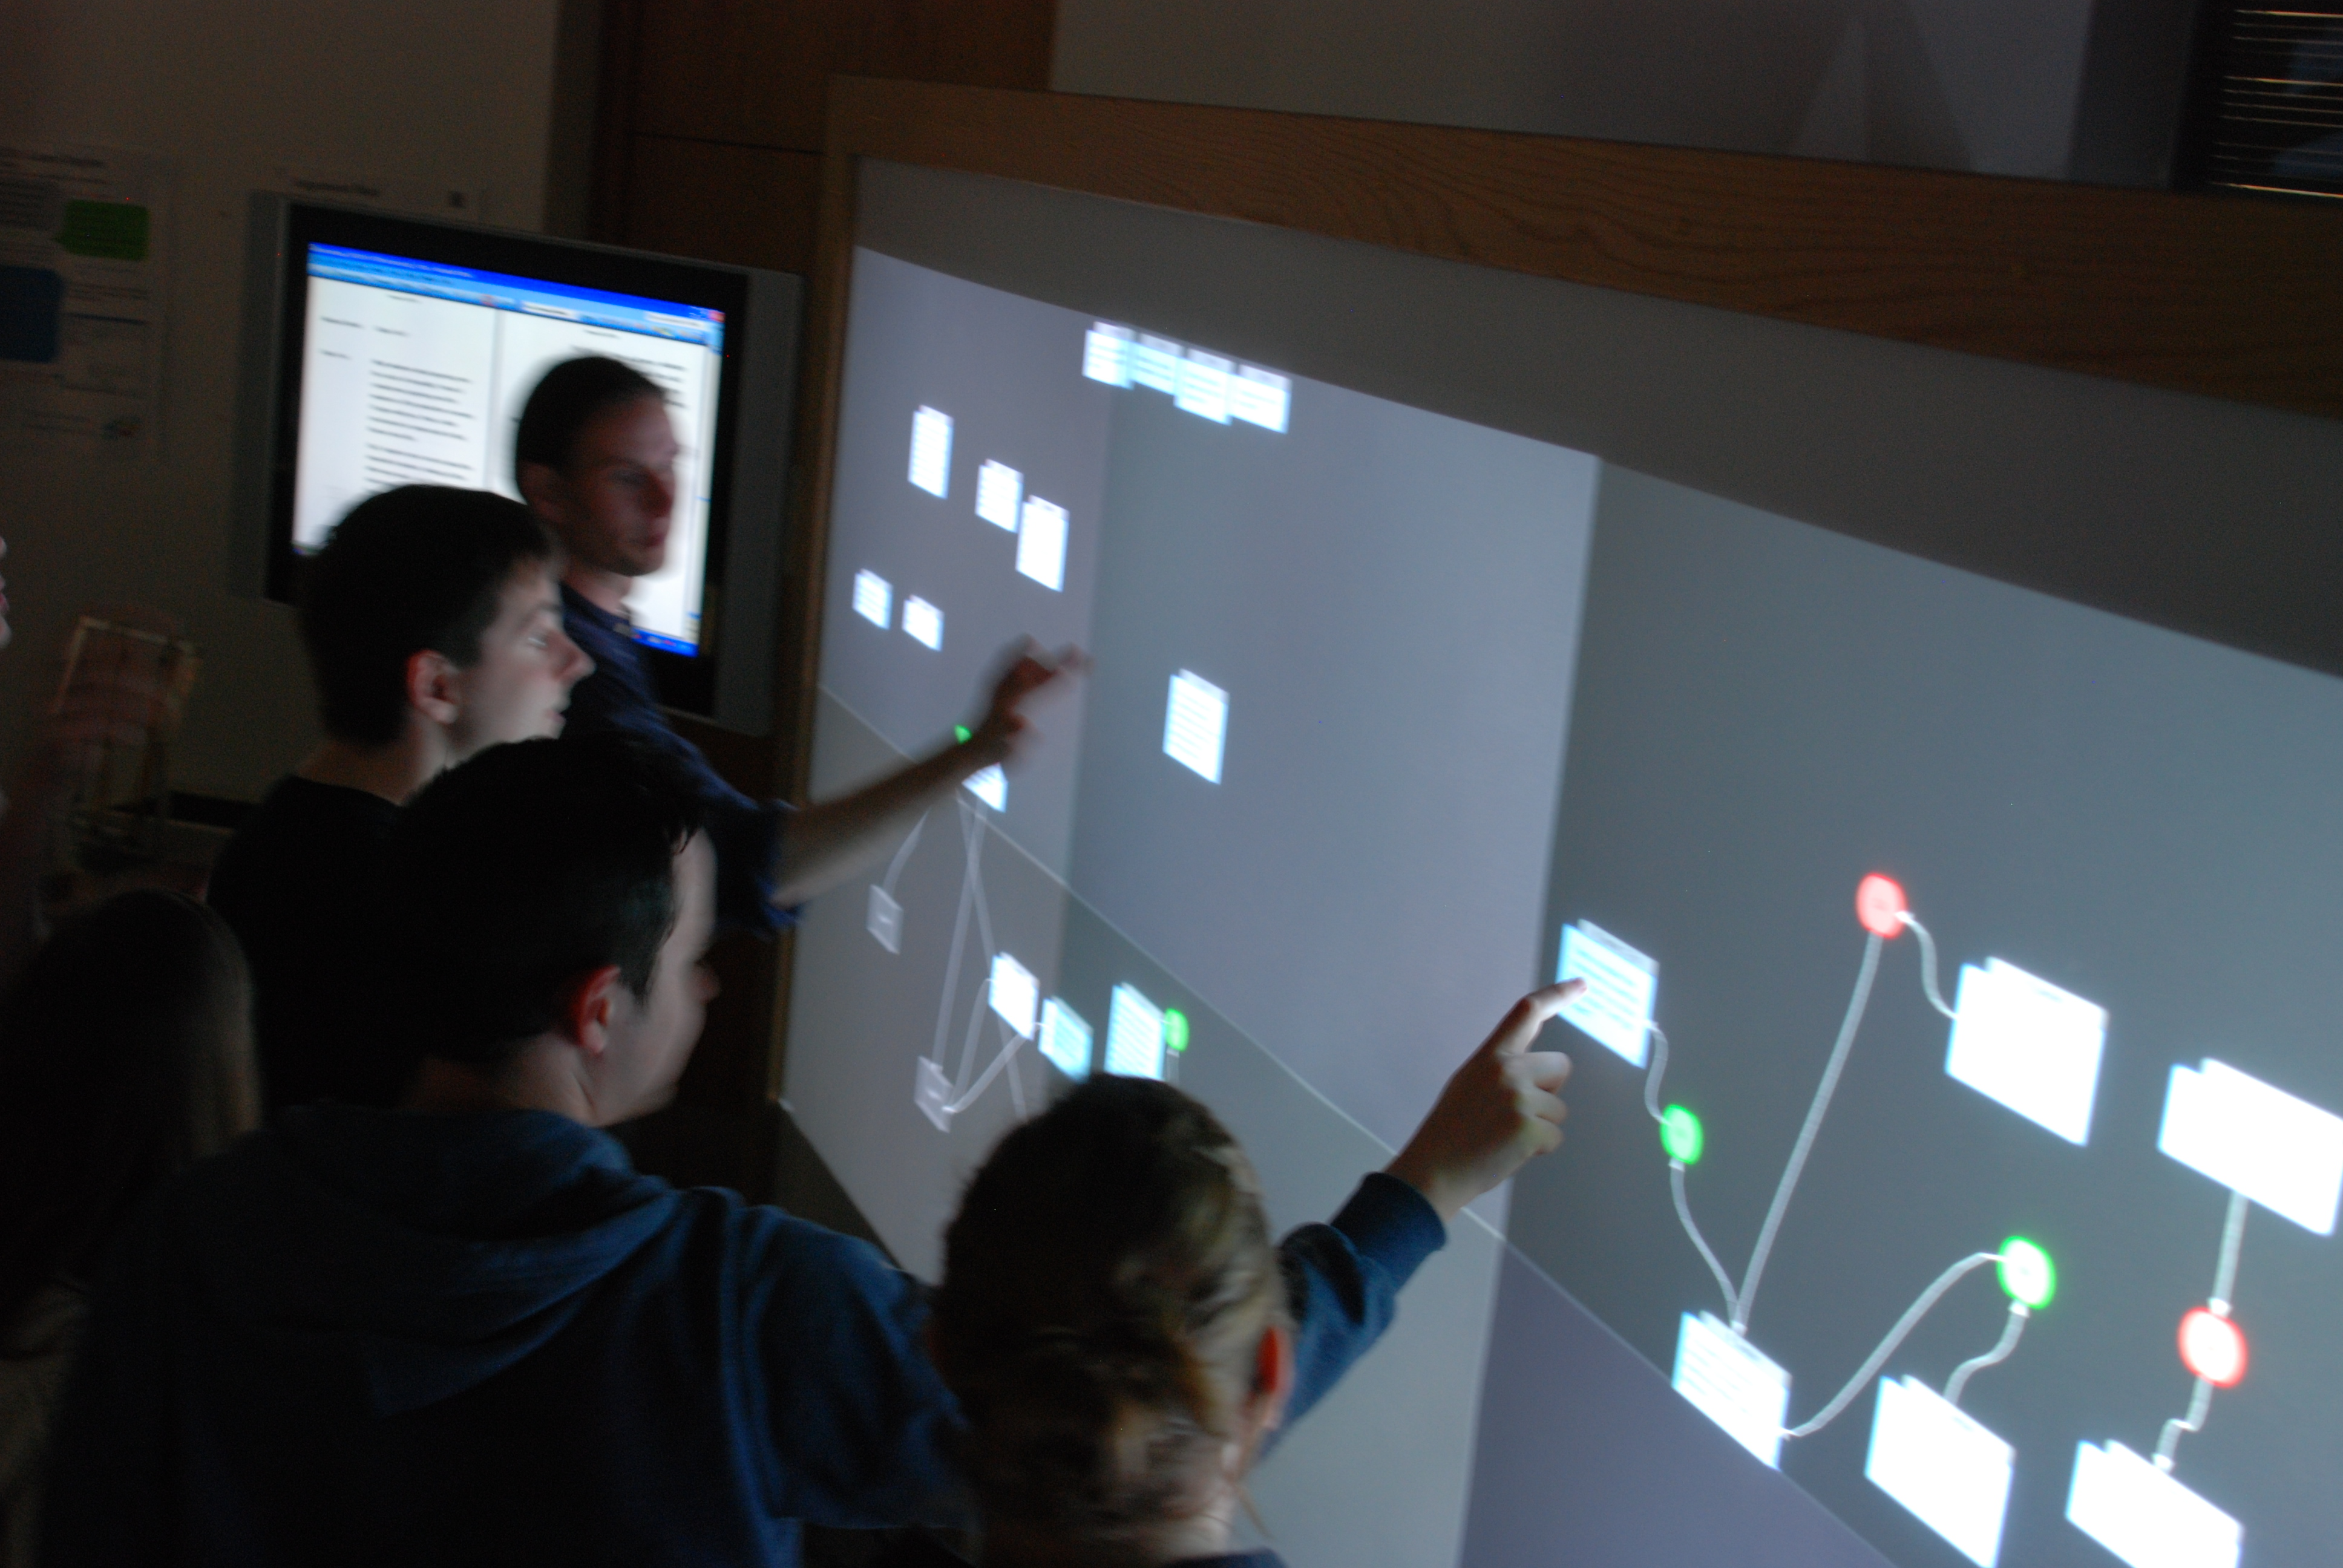
\includegraphics[scale=0.4]{analysis_wall.jpg}
\caption{Anotacija pomoću AnalysisWall-a}
\label{fig:analysiswall}
\end{figure}

Analiza argumentacije u stvarnom vremenu moguća je uz alat AnalysisWall.
\footnote{7.1.2018. više o projektu na \url{http://www.arg-tech.org/index.php/projects/argument-analysis-wall/}}
Uz AnalysisWall moguće je analizirati debatu, prepoznavati i povezivati argumente 
koristeći video zaslon na dodir. 
